\documentclass[12pt]{article}


\usepackage[numbers]{natbib}
\usepackage{graphicx} 
\usepackage{amssymb, amsmath, amsthm} 
\usepackage{fontenc} 
\usepackage{amscd,latexsym,amsfonts,amstext,amsbsy}
\usepackage{euscript} 
\usepackage{enumerate} 
\usepackage{color}  
\usepackage{physics}
\usepackage[latin1]{inputenc}
\usepackage{tikz}
\usepackage{mathrsfs}
\usetikzlibrary{shapes,arrows}
\usepackage{multicol}
\usepackage{comment}
\usepackage{color,soul}
\usepackage{combelow}
\bibliographystyle{apa}
\definecolor{applegreen}{rgb}{0.55, 0.71, 0.0}




\textwidth = 16 cm
\textheight = 24 cm
\oddsidemargin = 0.0 cm
\evensidemargin = 0.0 cm
\topmargin = -2 cm
\parskip = 0.2in
\parindent = 0.0in


\newtheorem{theorem}{Theorem}
\newtheorem{problem}[theorem]{Problem}
\newtheorem{exercise}[theorem]{Exercise}
\newtheorem{corollary}[theorem]{Corollary}
\newtheorem{lemma}[theorem]{Lemma}
\newtheorem{proposition}[theorem]{Proposition}
\newtheorem{proporties}[theorem]{Proporties}
\newtheorem{definition}[theorem]{Definition}
\newtheorem{definitions}[theorem]{Definitions}
\newtheorem{example}[theorem]{Example}
\newtheorem{remark}[theorem]{Remark}

 


\begin{document}
\textbf{\large{Modeling the Heroin Epidemic}} \\
Suzanne Lenhart, Tricia Phillips, Christopher Strickland \\

\textcolor{blue}{Blue font: contains questions I have, things to discuss.} \\
\textcolor{red}{Red font: things I am working on/need to do.} \\ \\
\textbf{Abstract} \\ \\
\textcolor{red}{Fill in after write paper.} \\ \\
\textbf{Introduction} \\ \\
\textcolor{blue}{Unsure of which pieces to take out/are unnecessary, so I labeled the main ideas of the paragraphs.} \\ \\
\textcolor{green}{Heroin information} \\ \\
\textcolor{blue}{About the drug: I think most of this can be taken out?} \\
Heroin is an illicit drug classified as an opioid and comes in the form of a white or brown powder or as a black substance resembling roofing tar. The drug is injected, sniffed, snorted or smoked and quickly enters the brain to bind to opioid receptors. It provides the user with feelings of euphoria, in addition to physical effects such as heavy feelings in the arms and legs, dry mouth, and sometimes nausea and vomiting \cite{NIH1, NIDA2}. There are short and long term negative effects on the body for using the drug, and consequently, it is currently considered a schedule I drug, meaning that there is no approved medical use of heroin and there is a high likelihood for abuse. \cite{DEA1, NIH1}. Addicted individuals have withdrawal symptoms such as restlessness, diarrhea, vomiting, and cold flashes, along with cravings for the drug which makes stopping use of the drug very difficult \cite{NIH1}. Options for treatment for heroin use involve medications such as buprenorphine, methadone, and naltrexone, in combination with counseling and behavioral therapies \cite{SAMSHA1, NIH1}. Heroin users build up a tolerance to the drug with repeated use and can overdose on the drug, in which their heart rate and breathing is slowed to a dangerous level without medical assistance \cite{NIDA2, NIH1}. Due to built-up tolerance, the risk of overdose is high when individuals stop their use of the drug for a period of time (i.e. while in recovery or hospitalized) and return to use. This is because they may return to the previous amount they were taking before, without knowing what their body can currently tolerate \cite{NIH2}.  

\textcolor{blue}{Statistics regarding heroin and why we should care:} \\
A national survey estimated that out of the United States national population of individuals 12 years of ago or older, 948,000 were heroin users in 2016, although this number may include under-reporting \cite{CDC2}. There were an estimated 13,219 heroin deaths in 2016, a more than six-fold increase from the year 2002, despite there being roughly half as many heroin users in 2002 \cite{NSDUH1}. This, in part, is due to the recent trend of lacing heroin with fentanyl, a surgical-grade opioid that is up to fifty times more potent than heroin alone, and therefore, users are unaware of the purity of the heroin they obtain \cite{CDC1, NIH2, Volkow2}. The effects of heroin, however, extend further than just the using individual. Due to the sharing of needles and other equipment involved in the injection of heroin, the human immunodeficiency virus (HIV) and the hepatitis C virus (HCV) are more easily contracted as transmittance occurs through bodily fluids. Moreover, risky sexual behavior is more likely under the influence, so for those whose method of use is via smoking or snorting, there is also an increased risk of transmitting and contracting these viruses. Women who use heroin during pregnancy put their babies at risk for neonatal abstinence syndrome in which the drug is passed along to the baby, resulting in dependency and thus, withdrawal symptoms upon birth \cite{NIDA2}. 

\textcolor{blue}{Heroin history: I think this can be taken out?} \\
Heroin was first formulated in a hospital in 1874, but production on a commercial level did not begin until 1898, when the Bayer Company in Germany marketed and sold the new drug. Prescription heroin was deemed helpful for treating bronchitis, asthma and tuberculosis, but near the turn of the century, the dangers of the drug were starting to be revealed, such as it's potential for addiction. In 1920, the American Medical Association stated that heroin should not be manufactured, sold, or prescribed in the United States, and in combination with the amount of crime resulting from heroin use, a law was passed in 1924 prohibiting crude opium imports with the intention of heroin production. With the start of World War II, traffickers diluted the drug more and more, due to tighter border controls and fewer supplies entering the country \cite{UnitedNations}. \textcolor{red}{More heroin history: find reliable source for smuggling of heroin from China to US in 1930s; motor vehicle vs. drug overdose stats; ~750,000 heroin addicts from 1965-1970; purity level/price of heroin; provide argument for why the problem is so large now that we need data-driven models compared to just a theoretical heroin addiction model as done for decades.} 

\textcolor{green}{Fentanyl information} \\
\textcolor{red}{Put in background on fentanyl.} \\

\textcolor{green}{Prescription opioid information} \\
\textcolor{blue}{About prescription opioids and why we should care:} \\
Another large portion of opioids consist of prescription pain relievers which are either natural, such as morphine and codeine, semi-synthetic, such as oxycodone, hydrocodone, and oxymorphone, or synthetic, such as fentanyl and tramadol \cite{CDC3, TNMentalHealth2}. From 1991 to 2011, there was a near tripling of prescriptions that pharmacies distributed \cite{NIDA1}. This was in part due to a number of new opioids that were approved by the FDA for use, such as OxyContin, Actiq, Fentora, and Onsolis (fentanyl), in addition to other unapproved opioid products for pain management \cite{FDA1}. Moreover, in the early 2000s, drug manufacturers funded publications and physicians to support opioid use for pain control \cite{Mandell}. A national survey estimated there were 11.5 million individuals 12 years of age or older in the United States that experienced pain reliever misuse in the past year, referring to the year 2016 \cite{CDC2}. In this survey, misuse was defined as taking the prescription at a higher dose, more frequently or longer than prescribed, taking someone else's medication, or any other way not directed by a doctor \cite{SAMSHA3}. This subset of the opioid drug class is misused for a variety of reasons and the same survey asked individuals who reported prescription pain reliever misuse to give the reason and the source for their most recent misuse. The most prominent responses for reasons of misuse were to relieve physical pain, to feel good or get high, and to relax or relieve tension. The largest source was from friends/relatives or from a healthcare provider, followed by given a prescription or stolen from a health care provider \cite{CDC2}. Treatment options for opioid addiction are the same as heroin \cite{SAMSHA1}. In addition, pregnant women who take prescription opioids also put their babies at risk of neonatal abstinence syndrome, similar to heroin \cite{CDC5}. 

\textcolor{blue}{I left out the prescription opioid ``history" since was covered in opioid paper and not as much of our focus?}

\textcolor{green}{Connection between opioid and heroin abuse} \\ \\
\textcolor{blue}{Transitioning from prescription opioids to heroin:} \\
The misuse of prescription pain relievers leads some individuals to start heroin. According to the National Survey of Drug Use and Health (NSDUH) survey information from 2002-2011, nearly 80\% of heroin users reported non-medical prescription pain reliever use prior to their heroin use. Here, non-medical prescription use is defined as taking prescriptions that were not prescribed to the user directly or used only for the feelings it causes. In fact, those who had prior non-medical prescription pain reliever use were 19 times more likely to initiate heroin use than those without prior use \cite{Muhuri}. This could in part be due to the higher availability of heroin in recent years at a lower cost than alternative opioids \cite{NIDA1}. Moreover, approximately 3.6 percent of non-medical prescription pain reliever users began using heroin within 5 years of their first opioid; although a small percentage, this is a significant number of individuals given the magnitude of opioid addiction \cite{Muhuri}. In 2010, an abuse-deterrent formulation of the commonly abused prescription opioid OxyContin was released that made abuse through injection and inhalation more challenging. Although done with the intent of reducing opioid abuse, studies showed that many individuals switched to heroin use instead \cite{Cicero2, Cicero3}. One study of young adults ages 18-25 concluded that among many factors including race, education status, martial status, other drug use, as well as many others, the use of non-prescribed opioid pain relievers in the past year was the biggest indicator of an individual using heroin in the past month, past year or in their lifetime \cite{Ihongbe}. Comparing NSDUH data from 2002-2004 and 2008-2010, the average yearly rates of past year heroin use increased among non-medical opioid users, but heroin use stayed static for those who reported no non-medical use of opioids; the highest rate of heroin use was among individuals with past year non-medical use of opioids ranging between 100 and 365 days of use \cite{Jones}. In the 1960's, heroin users were composed mainly of younger, nonwhite men in urban areas with their initial opioid being heroin, but in recent decades, this trend has shifted to older, white, rural and suburban men and women with their initial opioid being a prescription \cite{Cicero}. Opioids are of no shortage in society today and since opioid addiction is driven largely by legal prescription medication availability, this has made a significant proportion of society susceptible to misuse and addiction to opioids, including heroin. 
\textcolor{blue}{Add more in here from background papers?}\\ 


\textcolor{green}{Goal paragraph} \\ \\
\textcolor{blue}{Goals for our model/questions trying to answer:} \\
The misuse of opioids, including prescription pain relievers, synthetic opioids, and the illegal drug heroin, is rampant in today's society \cite{NIH2}. The opioid crisis was declared a public health emergency in October 2017 by the United States Department of Health and Human Sciences \cite{HHS1}. It was estimated that the total economic cost of prescription opioid dependence, abuse and overdoses in 2013 alone was \$78.5 billion \cite{Florence}. Due to the health risks of the addicted individuals, public health concerns, the number of overdose deaths and the economic burden, this is an issue worth paying attention to.
To address this apparent problem in today's society, we wish to model the prescription opioid/heroin/fentanyl epidemic in order to understand the dynamics behind the epidemic and predict the trajectory of the epidemic. We also wish to identify important conditions relating to the reduction of opioid/heroin/fentanyl addiction. To do that, we have formulated a population level system of ordinary differential equations model consisting of classes of individuals taking prescription opioids, addicted to opioids, using heroin or fentanyl, and successfully recovered from addiction to opioids, heroin and/or fentanyl, and analyzed it. Our overall goal is to explore how different management strategies may alter the epidemic trajectory; specifically, we would like to investigate management strategies for optimally treating pain with prescriptions while reducing opioid, heroin, and fentanyl addiction.

\textcolor{green}{Other models} \\ \\
\textcolor{blue}{Previous models involving heroin: should I do fewer details/group similar models while talking about them?} \\
There have been several models formulated focusing on heroin addiction. Most of them were motivated by and extensions of the White and Comiskey ordinary differential equation model with three compartments each representing a different stage as a drug-user: the susceptible class including individuals aged 15-64, the drug user class composed of individuals not in treatment, and finally, the drug users in treatment. In this model, individuals in treatment for drug use were only able to die, relapse to drug use, or complete treatment and be immune to drug use for the remainder of the modeling time period. The basic reproduction number, $\mathscr{R}_0$, was calculated and deemed most sensitive to the rate of individuals in the susceptible class becoming drug users; therefore, prevention is more important than treatment for reducing drug use \cite{White}. Wang, Yang and Li did analysis of this model, changing the assumption that the population was not constant \cite{Wang}. 

%\textcolor{blue}{Question: How can the model assume the three compartments make up the entire population, but then have the option for immunity to drug addiction for the remainder of the modeling period? Answer: NOT necessarily the same people; just equal number of people (i.e. someone is born susceptible to replace someone who became immune, maybe)  

The White and Comiskey model was modified later on by Liu and Zhang in order to incorporate a relapse distribution in which there was a non-constant time to relapse. They formulated a delay-differential equation, and also took away the assumption that the population was constant. Their conclusions about the sensitivity of $\mathscr{R}_0$ to certain parameters were in line with those from White and Comiskey \cite{Liu}. Using the same three compartments, another model was formulated with the idea of the relapse rate relying on the length of time the individual has been undergoing treatment. This coupled ODE-PDE model assumed that susceptibles could only become addicted via interaction with heroin users not undergoing treatment. Prevention was deemed more important than treatment, yet again \cite{Fang1}. Fang, Li, Martcheva and Caialso (2015) also modeled the heroin epidemic allowing susceptibility of becoming a drug user to depend on age, again resulting in a coupled ODE-PDE model \cite{Fang2}. A non-autonomous version of the White and Comiskey model included a distributed time delay for becoming a drug user along with both the parameters and the total high-risk population size being time-dependent \cite{Samanta}. From this, an autonomous model was developed incorporating the distributed time delay, which was converted into a discrete model with the time step-size being one \cite{Abdurahman}. Finally, a three compartment model consisting of susceptibles, users not in treatment, and those in treatment, assumed that those not in treatment could not recover and return to being susceptible, and that it took two contacts with a drug user to become addicted, resulting in a nonlinear incidence rate; results showed that perhaps the heroin prevalence undergoes periodic changes depending on conditions \cite{Ma}. 
%\textcolor{blue}{Question: Should I go through each paper specifically, like I have above, or moreso "group them" by stating some ways that the White and Comiskey model was modified and then reference them all together?} Answer: do them individually, that's better 

A deviation from the three compartmental model was done that included a fourth compartment which consisted of individuals who successfully recovered from their heroin use, whether through deciding to stop use by themselves or via treatment measures. The treatment of heroin users is limited by the availability of treatment facilities and resources and therefore, a saturated treatment function is incorporated; the saturation parameter was concluded as having the most vital role in the persistence of the epidemic. This implies that intervention is important early on before heroin addicts accumulate in the community and thus, prompt treatment is necessary \cite{Wangari}. 
 %http://journals.plos.org/plosone/article/file?id=10.1371/journal.pone.0102263&type=printable) 
Another model consisting of 84 ODE's captured the dynamics between prescription opioid users with acute pain, those with chronic pain, illicit opioid users, heroin users and those who overdose. Results showed that increasing addiction treatment and reducing prescriptions for individuals with chronic pain seemed to have a greater impact on reducing both heroin overdose deaths and the number of opioid abusers compared to reducing prescriptions for acute pain without treatment increases \cite{Benneyan}. \textcolor{red}{This was from a conference preceding...in future, look for published model from Benneyan.} 

%\textcolor{blue}{Question: Should only include population level models, correct...not something like a heroin market model (agent-based) with drug users, sellers, homeless \& police?} Will put in that model, and can do anything related because if those authors are editors, they will not like if they don't see their own work referenced. 

Others have taken a completely different approach, specifically using agent-based modeling. In addition to their ODE model, Benneyan, Garrahan, Ilie\cb{s}, and Duan (2017) formulated two agent-based models: the first being a cellular automata model consisting of a grid with neighboring cells updated depending on state variables adjacent to the cells; the second being a network model with nodes that represent individuals/subpopulations and weighted pathways dependent on relational strength and nearness. \textcolor{red}{Not all variables are defined, such as P(x,y), so look for full model from Benneyan when published.} The former was to better understand regional spread and the latter to investigate spread among individuals; their results suggested that with various regulation practices for opioids, heroin death rates would decrease, but the authors recognize the reality of unintended consequences of these legislations \cite{Benneyan}. Agar (2001) created an agent-based model, consisting of a world with 2,500 patches and 100 agents each assigned an experimentation value which defines how likely that individual is to experiment with heroin, depending on their interest in trying something new, their attitude toward illicit drug use, and their desire to follow societal rules. The model was able to track the number of heroin experimenting individuals over time with the agent moving randomly, one patch selected at random to contain heroin in the beginning, and the ability for individuals to obtain heroin from their original patch, from others who have experimented, or from another patch where the transferring of heroin between agents occurred \cite{Agar}. \textcolor{red}{Put in brief explanation of ``Reducing the complexity of an agent-based local heroin market model" paper by Heard. \\ Look up if any models out there regarding fentanyl use/addiction.} \\

\textcolor{blue}{Summary of Christopher's opioid paper and why formulating another model:} \\
\textcolor{red}{Need to update with new revisions/any new results from final version that's published!} The motivation for our heroin model came from a previous model focusing on opioid addicts through prescriptions or via the black market \cite{Battista}. In order for the model to have an addiction-free equilibrium, both addictions that come from prescriptions and addictions from accessibility to excess prescription drugs must be eliminated, which equates to the need for close administration and monitoring of those prescribed. Furthermore, near the addiction-free state, the prevention of prescription opioid users becoming addicted is more important for staying near the addiction-free equilibrium than reducing the number of prescriptions getting into the hands of non-prescribed users. However, away from the addiction-free state, a realistic situation, the most important factors in reducing the number of addicted individuals include increasing the prescription completion rate, increasing entry into treatment (even among low success rates), and decreasing the prescription rate. The purpose of formulating a separate model from this prescription opioid model is to be able to understand the more complicated dynamics that arise among opioid addiction with the addition of heroin/fentanyl use. As exemplified previously, heroin and fentanyl play a significant role in the process of opioid addiction and recovery and so it's inclusion provides a more accurate overall picture of the epidemic. In addition, since heroin users overdose almost as much as prescription opioid users and in recent years, a sharp increase of heroin overdoses has occurred primarily due to the involvement of fentanyl, it is crucial to take a more detailed look at this increasing problem \cite{CDC4}. Moreover, we wish to alter how the recovery process is viewed, by thinking about those in recovery still as addicts, and not having the ability to become a susceptible individual again. 




\textcolor{blue}{How our model is different than previous models:} \\
\textcolor{red}{Include details on how my model different than previous ones.} Previous models have not incorporated the connection between prescription opioid misuse and heroin or fentanyl use at all, instead focusing solely on heroin addiction and recovery. Although there are many factors that play a role in population size, susceptibility to drug use, relapse time and other parts of the drug-using process, we consider individuals in each of the classes to be homogeneous, for simplicity of a starting model. \textcolor{blue}{Can I say: discussion of how our model differs from the prescription opioid model (Christopher's) will be discussed after the description of the model to be able to give more specific details?}


\textbf{Model Formulation} \\ \\
To the extent of our knowledge, there have been no mathematical models incorporating both prescription opioid use and heroin/fentanyl use. Our model consists of five subgroups of the Tennessee population, in which they are all proportions of the entire population: 

1. Susceptibles ($S$): This portion of the population consists of individuals who are not taking prescription opioids of any kind, nor using heroin or fentanyl. \\ \\
2. Prescription opioid users ($P$): This class of individuals consists of individuals who are prescribed opioids by a health care provider and take the opioids at a level that is not considered addicted. We note that individuals in this class could be misusing prescription opioids, but not at the level of addiction.  \\ \\ %"Misuse" in data: questions may ask about misuse in the past 12 months, and so even 1 time of misuse would count 
3. Opioid addicts ($A$): This group of individuals are addicted to opioids, but not using heroin or fentanyl, or are actively in treatment for opioid addiction, or are within 4 weeks post-treatment for opioid addiction. (Although the opioid class of drug includes heroin and fentanyl, here we will take opioids to mean non-heroin and non-fentanyl.) \\ \\
4. Heroin/fentanyl users ($H$): This class is composed of individuals who are addicted to heroin or fentanyl or are actively in treatment for heroin/fentanyl addiction, or are within 4 weeks post-treatment for heroin/fentanyl addiction. We note that individuals in this class could be using other drugs or are addicted to opioids in addition to heroin or fentanyl, but they are at least addicted to one of these drugs. \\ \\
5. Recovered individuals ($R$): This class consists of individuals who completed treatment for opioid or heroin/fentanyl addiction and did not relapse within 4 weeks post-treatment, and therefore are considered in a ``stable/successful" state of being recovered. We make assumption that those in the recovery class are not considered addicted. \textcolor{red}{I believe ROSIE study says somewhere that individuals in treatment are mostly still taking drugs, which supports our decision to leave those in treatment in an addicted class: https://www.drugsandalcohol.ie/11542/1/ROSIE3-YearReport.pdf} \\

\textcolor{blue}{Clarifications on definitions:}
We assume that these five compartments sum to one, so that the population is of constant size, i.e. the total death rate is equal to the incoming rate for the susceptible class. Although terminology is not always clearly defined in the literature, such as opioid misuse, abuse, dependency, addiction and use disorder, we aim to focus on addiction only, where addiction to opioids is defined as having a pattern of continued non-medical use that is already, or could be, harmful \cite{Vowles}. We take opioid use disorder to fall in this categorization of addiction, due to the definition presented in \cite{SAMSHA2} which includes sustained use regardless of interference with life obligations. We include illicit fentanyl users in the class of heroin users, because of the potency of the drug, which is what those addicted to prescription opioids seek--lower cost and a better high. In addition, a portion of those who overdose from the very powerful drug fentanyl are individuals who are using heroin that is laced with it; therefore, the use of fentanyl is oftentimes intertwined with the use of heroin. There is much variability in the purity of heroin due to the lacing of the drug with fentanyl, and 1 in 5 overdose deaths have multiple drugs present so it is difficult to know the actual cause of death \cite{CDC4}. We believe it is difficult to separate the use of heroin and fentanyl, so putting them in the same class seems the most natural choice. Finally, we remark that use of heroin is implicitly understood to be addictive due to the highly addictive nature of the drug, and we assume no casual or recreational use of the drug \cite{NIH1}. If an individual were to use heroin and it was easy to stop (i.e. not addicted), although seemingly unrealistic, we think they are better classified as a susceptible individual. Similarly, use of fentanyl outside of a short-term, carefully monitored setting by a health provider most likely equates to addiction. \textcolor{red}{Source for fentanyl addictive nature, length of time of prescription short?} We try to take into account these complexities as best as possible with the information in literature.


We will run our model from 2013-2017, and initial conditions for the classes will be estimated, as we do not have data for the number of individuals in each class at the beginning of 2013.  
We denote the initial conditions as
$S(0)=S_{0}$, $P(0)=P_{0}$, $A(0)=A_{0}$, $H(0)=H_{0}$, and $R(0)=R_{0}$, and we assume all of these values are positive. The initial values for each of the classes are proportions of the entire population and therefore are dimension-less.

 
Here, we present our ordinary differential equation model: %without delta
\[\dv{S}{t} = -\alpha S - \beta_{A} SA  -\beta_{P} SP- \theta_{1} SH +\epsilon P +\mu (P+R) + (\mu+\mu_{A})A + (\mu+\mu_{H}) H \quad (1)\] 
\[\dv{P}{t} = \alpha S - \epsilon P  - \gamma P - \theta_{2}PH- \mu P    \quad(2)\]
\[\dv{A}{t} = \gamma P + \sigma R \frac{A}{A+H} +\beta_{A} SA  +\beta_{P} SP -\zeta A - \theta_{3}AH-(\mu + \mu_{A})A   \quad (3)\]
\[\dv{H}{t} = \theta_{1}SH+\theta_{2}PH+\theta_{3}AH + \sigma R \frac{H}{A+H}-\nu H-(\mu+\mu_{H})H  \quad (4)\]
\[\dv{R}{t} = \zeta A +\nu H -\sigma R \frac{A}{A+H}-\sigma R \frac{H}{A+H} -\mu R\quad(5).\]


The parameters involved in this model represent transition rates from one class to another and are per capita yearly rates; specifically: 
\begin{itemize}
\item $\alpha S$: rate at which susceptible individuals are prescribed opioids (1/year)
\item $\beta_{A} SA$: rate at which susceptible individuals become addicted to opioids by black market drugs or interaction with other addicts (1/year)
\item $\beta_{P} SP$ : rate at which susceptible population obtains extra prescription opioids and becomes addicted  (1/year)
\item $\theta_1 SH$: rate at which susceptible population becomes addicted to heroin or fentanyl by black market availability or interaction with other heroin or fentanyl users  (1/year)
\item $\epsilon P$: rate at which individuals return to the susceptible class after being prescribed opioids and did not develop an addiction (1/year) 
\item $\mu S, \mu P, \mu A, \mu H, \mu R$: natural death rates (1/year)
\item $\mu_A A$: enhanced death rate for opioid addicts; overdose rate which results in death (1/year)
\item $\mu_H H$: enhanced death rate for heroin or fentanyl addicts; overdose rate which results in death (1/year)
\item $\gamma P$: rate at which prescribed opioid users become addicted to opioids (1/year)
\item $\theta_2 PH$: rate at which prescribed opioid users become addicted to heroin or fentanyl (1/year)
\item $\sigma R \frac{A}{A+H}$: rate at which individuals transition from the recovered class into the opioid addicted class which is proportional to the approximate proportion of individuals in the recovered class that came from A that are relapsing back to that class. (note: even though we do not know where individuals came from originally, we make the assumption that individuals go back to their primary drug of choice/the reason they entered treatment, so relapse back approximately proportional to where they came from \textcolor{red}{Find source, or assume they do for simplicity.}) (1/year)
\item $\zeta A$: rate at which addicted opioid users enter treatment/rehabilitation (1/year)
\item $\theta_3 AH$: rate at which the opioid addicted population becomes addicted to heroin or fentanyl  (1/year)
\item $\sigma R \frac{H}{A+H}$: rate at which individuals transition from the recovered class into the heroin/fentanyl addicted class which is proportional to the approximate proportion of individuals in the recovered class that came from A that are relapsing back to that class. (note: even though we do not know where individuals came from originally, we make the assumption that individuals go back to their primary drug of choice/the reason they entered treatment, so relapse back approximately proportional to where they came from \textcolor{red}{Find source, or assume they do for simplicity.}) (1/year)
\item $\nu H$: rate at which heroin or fentanyl users enter treatment/rehabilitation 
\end{itemize} 
%Recovery--1 month: those in treatment experience acute withdrawal, after 1 month: post-acute (emotional freight train) 
%potentially make theta1=theta2 to reduce the number of parameters
%Look at pain management articles and why people relapse. 
%Get intuition about potential arrows from papers. 

\textcolor{blue}{Clarification of some aspects of the model:} \\
Since susceptible individuals die and give birth at the same rate, $\mu S$, those terms do not appear in the differential equation for susceptibles. Also, we note that although sellers are not directly involved in the model nor have to be addicts themselves, addicted individuals act as a proxy for sellers of the drug and general availability of the drug, whether it is opioids or heroin. This is because the higher number of addicted individuals there are, the more sellers there needs to be which results in an increased exposure to the drug and therefore, increased chance of addiction. Although treatments for addictions are an enormous problem in and of themselves since there is limited success as shown by the parameter values for the recovery rates, we are incorporating treatments at a shallow level as a part of our model. We are classifying overdoses to mean opioid overdose-related deaths (i.e. not from secondary factors or long term effects). We note that although overdose death data includes both accidental and non-accidental deaths (i.e. suicide, assault), we assume that if an individual died from an opioid overdose-related death, they were addicted to begin with and unintentionally overdosed, and that the number of intentional overdoses is negligible. \textcolor{red}{This is CDC definition (from data packet) is for prescription opioids and fentanyl; see if also same for heroin.}
%https://pep-c.rti.org/HERO/KB/Documents/CDCs\%20Opioid\%20Overdose\%20Indicator\%20Support\%20Toolkit.pdf%
We also note the fact that Naloxone, an overdose-reversing medication, has saved individuals from overdoses, but \cite{NIDA2} \textcolor{red}{make some argument that the number saved is negligible compared to the number of overdoses, so we assume results in death most of the time.}\\ 

\textcolor{blue}{Explanation of R class/why, justification of 4 week mark, how different from Christopher's opioid paper:} \\
\textcolor{red}{*****Update from Recovery\_ideas.pdf explanations when finish.}\\
We note that the terms $\sigma R \frac{A}{A+H}$ and $\sigma R \frac{H}{A+H}$ were included in order to avoid having two recovered classes, which would prevent the transition of individuals who recovered from one drug to initiate use of the other (or if we included those pathways, would become too complicated for a first model). One study suggested that 10\% of the prescription opioid addicts they followed up with post-treatment had used heroin at least five times in the previous year, which demonstrates the importance of keeping these transitions as possibilities \cite{Weiss}. We decided to define a recovered class instead of a recovery class as the model presented in \cite{Battista} did, because the recovery class would have consisted of two very different groups of individuals: those with a high chance of relapse (e.g. recently finished treatment) and those with a much lower chance of relapse (e.g. successfully finished treatment in the past and has remained free of addiction for a significant amount of time). In addition, since an estimated 91\% of opioid addicts in recovery relapse back to addiction within 8 weeks post-treatment and 70\% of heroin addicts relapse within 4 weeks post-treatment, we wish to keep these individuals in the addiction class since they have not fully ``recovered," i.e. at a point where they are less likely to fall back into addiction \cite{Weiss, Smyth}. \textcolor{blue}{Will be changed to 70\% for 4 weeks post-treatment for opioid addicts once \textcolor{red}{update from recovery\_ideas.pdf with assumption/source and also if use ROSIE source above about how those in treatment are still addicted.}} One of these studies showed that 92\% of individuals who relapsed after discharge had gone back to treatment prior to their follow-up interview, which conveys the more unstable nature of their recovery particularly within a few weeks of post-treatment (since that's when a majority of them relapsed) \cite{Smyth}. \\ This definition of the recovered class creates a compartment to put individuals who have been addicted in the past and have finished treatment but are not considered actively addicted anymore and should be dealt with differently than susceptible individuals, those in treatment, and those recently out of treatment. This definition of a recovered class is also beneficial when it comes to the data; data for the number of addicted individuals would include those in recovery, so our class avoids having to parse out how many are in recovery versus not in recovery.  \\ 

\textcolor{blue}{Explanation of pathways omitted:} \\
We omitted an interaction term between prescribed users and addicted individuals moving into the addicted class, under the assumption that since prescribed users have access to their own prescriptions to get addicted, they do not need an illicit source or interaction with addicts to become addicted themselves. Moreover, we did not include an interaction term RA to go from the recovered class to the opioid addicted class because we assume that individuals who are successfully recovered will not be influenced by addicts or by the general availability of the drug to fall back into addiction themselves. \textcolor{blue}{Currently working on these terms/ideas, so will most likely be updated.} We did not include an RH term from the recovered class to the heroin/fentanyl class for a very similar reason. We do not have a pathway from R to P; although individuals have the potential of obtaining a legal prescription from a doctor since doctors are not necessarily informed that their patient was in recovery in the past \textcolor{red}{find resource that talks about doctors being ``case-history blind"}, it does not seem realistic that an individual who has recovered from an opioid or heroin addiction would be able to successfully take prescription opioids in a non-addictive manner, and therefore would be in the addicted class almost immediately (there may be a few exceptions to this, but we will make this assumption for a first model).\\
%Only doing one term from A to H \sigma_2*A*H (different from two terms going from P to A because either become addicted to your own meds or interact with addicted people) because in order to start doing heroin, you HAVE to be in contact with someone who does (i.e. a dealer) so demand does play a role in how many people do heroin and therefore, how many go from A to H 


We omitted the pathway from R to S since individuals who have been to treatment and recovered are much more likely to fall into addiction than a susceptible individual, and therefore, must be treated differently than a susceptible individual who has not been to recovery (i.e. cannot be homogeneously mixed in S). We think of individuals in the recovered class as in a permanent state of recovery for the rest of their lives, although they are not undergoing active recovery, and we think of this class as an absorbing state. \textcolor{red}{Find source talking about addicted individuals who underwent recovery much more likely to fall back into addiction than susceptible individual...addiction being a disease.} Along these same lines, there is no pathway from A or H to S because we are under the assumption that an addicted individual will either remain addicted or go to recovery to help their addiction and will never be characterized as a susceptible individual again. We recognize that there may be additional pathways among the classes, but the ones we have chosen to include in our model are the ones we view as most important/realistic. \\ 

This compartmental model can be represented by the following flow diagram with each arrow representing either the transition rate between one class to another or birth/death: 

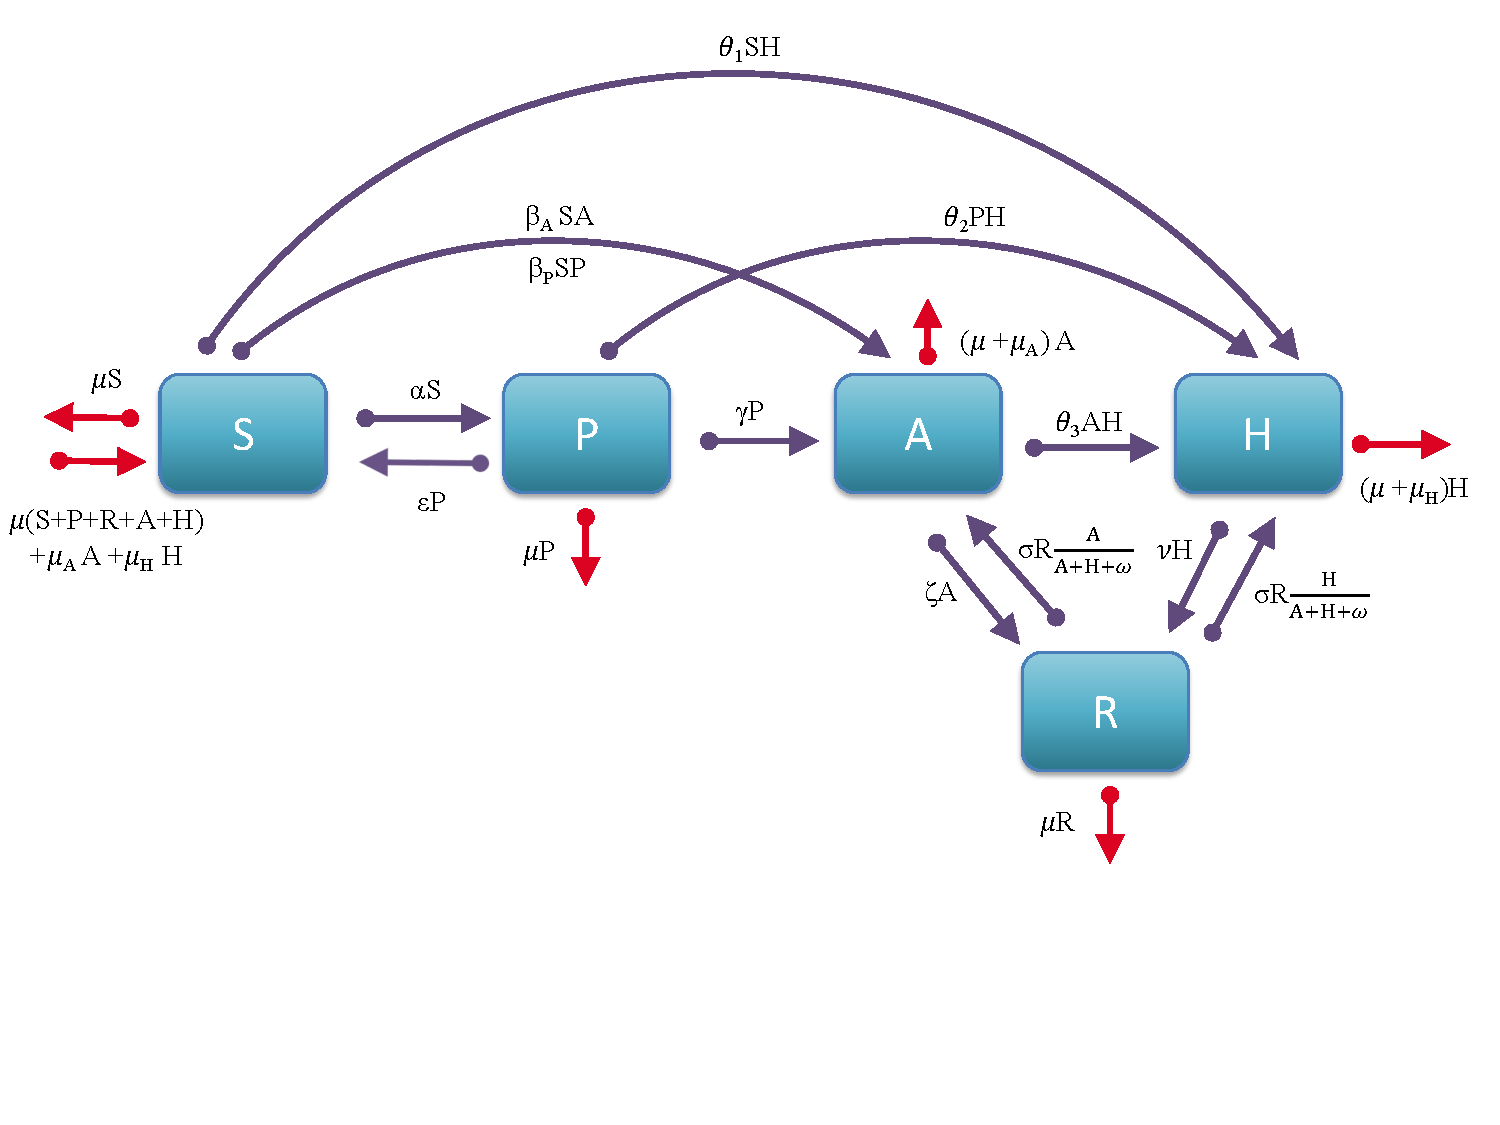
\includegraphics[scale=0.6]{heroin_schematic.pdf}
\vspace{-0.8cm}
\begin{center}
Figure 1: Schematic diagram for heroin model
\end{center}

%Christopher's words: (Regarding why we have so many assumptions). What can we say with a simple model? And from there, what can't we say? <-- This latter question gives us direction for how to improve the model and what we should do to build/extend the model further. 


\textbf{Analysis of the Model} \\ \\
\textcolor{red}{Fill in updated addiction-free equilibrium work.} \\
\textcolor{red}{Update basic reproduction number from new addiction-free equilibrium (if can).} \\  
\textcolor{blue}{Include proof of non-negative IC implies non-negative solutions?} \\ 
\textcolor{blue}{What other analysis should be done?} \\ \\
\textbf{Numerical Results} 
(literature information and parameter estimation) \\ \\
\textcolor{blue}{Parameter estimation codes using Ordinary Least Squares: HeroinModel.m, \linebreak HeroinModel\_ODE45.m, HeroinModel\_MultiStart.m ...with these 3 files open, can run by typing ``HeroinModel\_MultiStart.m" \\ \\
The parameter estimation codes right now reflect recent changes of the model (including the terms $\sigma R \frac{A}{A+H}$ and $\sigma R \frac{H}{A+H}$, but not with the perturbation term) and runs from 2013-2017. Currently we only have 7 data points and 15 unknowns, but 2 more data points can be put in once February reports come out for a total of 9 data points. If we run from 2015-2017, we would have 7 data points total and 12 unknowns. \\ \\
I tried to choose realistic lower and upper bounds for the parameters in the following way: $\alpha$ guess from opioid paper since higher in TN; $\beta_A $ guess from opioid paper; 
 $\beta_P$ guess from opioid paper; $\theta_1$ complete guess, assume smaller than $\beta_A$, $\beta_P$; 
 epsilon 0.8-8 from opioid paper; gamma guess from opioid paper; $\theta_2$
 guess twice as large as $\theta_1$; $\sigma$ guess small because
 ``successful recovereds"; $\zeta$ will be smaller than opioid paper because fewer people will ``relapse" since more ``stable recovered" but still
 put opioid largest value in; $\theta_3$ guess four times as large as
 $\theta_1$; $\nu$ guess same as $\zeta$; $P_0$
 guess; $A_0$ guess; $H_0$ guess; $R_0$ guess} \\ \\
 \textcolor{blue}{Could this info be used for relationship among $\theta_1$, $\theta_2$, and $\theta_3$?: Since we could not find data for values of $\theta_1$, $\theta_2$, or $\theta_3$ for Tennessee, we consider a national study of individuals 12 and older to establish a relationship among these three rates. For a national study consisting of 609,000 participants, ``the recent heroin incidence rate was 19 times higher among those who reported prior non-medical pain reliever (NMPR) use (0.39\%) than among those who did not report NMPR use (0.02\%) \cite{Muhuri}.
Thus, we will extrapolate this information to say that the rate that prescription opioid users and opioid addicts move to heroin use is 19 times greater than the rate at which susceptibles move to heroin use (i.e. $\theta_2 + \theta_3$ $>$ 19$\theta_1$).} \\

\textcolor{blue}{What other types of assumptions can we make regarding the parameters?} \\
 
 \textcolor{blue}{Data used within code:} 
 
1) For Tennessee, the \textbf{total number of individuals taking prescription opioids} for pain \cite{TNgov1}: \\
2013: 1,845,144 \\
2014: 1,824,342 \\
2015: 1,819,581 \\
2016: 1,761,363 \\
2017: 1,636,374 

Although this number does not explicitly state it is for individuals 12 and older, we assume it is since it comes from the Tennessee Department of Health; if it does include individuals under 12, we assume that number is negligible. In addition, we assume very few, if any, individuals are addicted to opioids outside of prescription opioids, but even if they are, we will assume they are taking prescription opioids in some capacity, so we will take pain reliever use disorder to include those with other non-prescription opioid addiction. \\

2) For Tennessee, the 2015/2016 average number of individuals 12 and older with ``Pain Reliever Use Disorder" (\textbf{opioid addicts}): 48,000 \cite{NSDUH2} \\
We note that their definition of pain reliever use disorder includes those who meet the American Psychiatric Association criteria for dependence or abuse. Here, opioid dependence is classified as having "signs and symptoms that reflect compulsive, prolonged self-administration of opioid substances that are used for no legitimate medical purpose or...are used in doses that are greatly in excess of the amount needed for pain relief...regular patterns of compulsive drug use that daily activities are typically planned around obtaining and administering opioids." This definition falls under our definition of opioid addiction. Opioid abuse, on the other hand, they consider to be less severe than dependence, and would not lead to the development of withdrawal symptoms. This latter definition does not fall under our characterization of addiction, but we make a note of this to say that this estimate for those with a pain reliever use disorder may be overestimated for what we are concerned with, but is an acceptable approximation \cite{DSM}. \textcolor{blue}{Right now, I'm using this estimate for the year 2015...should I compare it to total number in 2015+total number in 2016 divided by 2 instead?} \\

3) For Tennessee, the 2015/2016 average number of individuals 12 and older with ``Past Year Heroin Use" (\textbf{heroin/fentanyl addicts}): 14,000 \cite{NSDUH2}  \\ 
Although this number includes those who may have used heroin once or twice in the past year, we are under the assumption that the majority of these individuals are addicts and that very few, if any, individuals use heroin recreationally. In addition, the number of heroin users does not include fentanyl users explicitly, but we are under the assumption that those who take fentanyl are a subset of those who use heroin, and therefore, would mostly be included in these numbers. We admit the values may be slightly too low, for the cases of individuals who do fentanyl and not heroin, but data has not been found for fentanyl addicts only. Therefore, we are working under the assumption that it would be a negligible population that takes fentanyl without heroin. Overall, these two assumptions may work to balance one another out. 
\\

4) We use data on the number of prescription opioid overdose deaths which include natural, semi-synthetic, and synthetic opioids; however, we subtract out the number of fentanyl overdoses (fentanyl is classified as a synthetic prescription opioid), since those overdoses are counted for in their own category, listed below. This results in the following  \textbf{total number of prescription opioid overdose deaths} for 2015: (848-169=) 679 \cite{PDO}. Although this number does not explicitly state it is for individuals 12 and older, we assume it is since it comes from the Tennessee Department of Health; if it does include individuals under 12, we assume that number is negligible. \\

We add together the heroin and fentanyl overdoses for the state of Tennessee to obtain the \textbf{total number of heroin and fentanyl overdoses} in 2015 to be: (205+169=) 374 \cite{PDO}. Although this number does not explicitly state it is for individuals 12 and older, we assume it is since it comes from the Tennessee Department of Health; if it does include individuals under 12, we assume that number is negligible. \\

%SEE WORK on 11/19/18 meeting notes for mu_A, mu_H, mu
We may calculate the overdose death rate in the year 2015, since we know the number of addicted individuals in that year. To find the continuous-time rate at which individuals are dying from the addicted class, we consider the equation $k A_{0}=A_{0}e^{-\mu_{A}t}$, where $A_0$ is the number of individuals addicted to opioids in 2015 and $k$ is the proportion of these individuals in the addicted class at the start of 2016 (when $t=1$). In 2015, there were 679 individuals out of the entire Tennessee population 12 and older that overdosed on prescription opioids \cite{PDO}. However, it is estimated that only 54.6\% of these individuals were actually at an increased risk for an opioid-related overdose death; we will assume that if an individual met the criteria for at least one high-risk factor, that they were considered addicted to opioids \cite{Gwira}. Therefore, we will assume 54.6\% of the 679 individuals that overdosed were addicted. With a total of 48,000 opioid addicts in 2015, this means that (48,000-0.546$\cdot$679)/48,000 $\approx$ 0.992 is the proportion of addicted individuals that remain by the beginning of the next year. This implies 0.992$A_0=A_0 e^{-\mu_{A}(1)}$, and solving results in $\mu_{A} \approx 0.00775.$

Similarly, we may calculate $\mu_{H}$. There were 14,000 heroin/fentanyl addicts in 2015 and 374 heroin-related overdoses. We make the assumption that if an individual died of a heroin overdose they were addicted in line with our previous assumptions that if one is using heroin, they are considered addicted due to the nature of the drug. This means that (14,000-374)/14,000 $\approx$ 0.973 is the proportion of heroin users that remain at $t=1$, which implies 0.973$H_0=H_0 e^{-\mu_{H}(1)}$, which results in $\mu_{H}$ $\approx 0.0271$, the continuous-time rate at which individuals are dying from the heroin class.

%we view it as a good thing that methadone was pulled out separately from this data for overdoses, because it's used in treatment in order to reduce cravings and not necessarily supply the high 

We make a note that individuals that do not have an opioid use disorder and die because of an opioid overdose are counted in the ``natural mortality rate." \\

5) The total population estimates in Tennessee each year are the following \cite{USCensus}: \\
2013: 6,490,795 \\
2014: 6,540,007 \\
2015: 6,590,726 \\
2016: 6,649,404 \\
2017: 6,715,984 \\
2018: 6,770,010 

There were an estimated 1,073,214 individuals in Tennessee in 2018 aged 12 and under. (Note: we could not find the estimate for this age group for the years 2013-2017, so this is the best estimate we have for this age group). To figure out those who are 12 years old, we take approximately 1/8th of the individuals that are in the age group 5-12, which is approximately 83,175 individuals \cite{DOHHS}. Thus, an estimated 990,039 individuals are \emph{under} the age of 12 in Tennessee. Given the total population estimate for 2018 being 6,770,010 from above, this means that approximately 15\% of the population is under the age of 12. Since we do not see a reason for this percentage to be significantly different from year to year, we assume that this percentage is constant throughout the time period we are looking at. Then, we are able to consider the following \textbf{Tennessee population estimates for individuals 12 and older} in order to align with the rest of the data that is in this age range by taking off 15\% of the above total population estimates.  \\
2013: 5,517,176 \\
2014: 5,559,006 \\
2015: 5,602,117 \\
2016: 5,651,993 \\
2017: 5,708,586 

%Could be helpful if need for individuals under 12: https://factfinder.census.gov/faces/tableservices/jsf/pages/productview.xhtml?src=CF 
The \textbf{age-adjusted death rate} for Tennessee in 2016 was calculated to be 886.3 out of 100,000 individuals, or approximately 50,094 people out of a total population 12 and older of 5,651,993 \cite{Kaiser}. Subtracting off the number of people who died from a prescription opioid or heroin/fentanyl overdose in 2016 results in 48,825 people who died that year. This implies that (5,651,993-48,825)/5,651,993 $\approx$ 0.991 is the proportion of the population that remains by the beginning of 2017. If we consider $T_0$ to be the total population in 2016, we can find the continuous-time rate at which individuals die naturally from the equation 0.991$T_0$=$T_0e^{-\mu t}$, which results in the natural death rate $\mu \approx 0.00868$.


\textcolor{blue}{General explanation of parameter estimation process:} \\
In order to estimate parameters for our model, we used data regarding the proportion of prescription users, opioid addicts, and heroin/fentanyl addicts each year from above and compared these to the proportions of the population in the classes at in certain years that out model simulated. We estimated the following parameters: \textcolor{red}{fill in which ones, maybe referring to a table} and used the values calculated above for $\mu$, $\mu_A$, and $\mu_H.$ We ran the code from \textcolor{red}{fill in which years} with the time step in years. We utilized the ordinary least squares method and formulated an objective function to minimize, which consists of the squared differences between the data and model simulations. We used the optimization toolbox in MATLAB and specifically utilized the MultiStart algorithm and fmincon and used \textcolor{red}{fill in number} as the number of starting points to ensure that the global minimum is found, as this is a local solver. \\ \\
\textbf{Conclusions} \\ \\
 \textcolor{red}{What did we show that we didn't know before?}



\pagebreak

\bibliography{HeroinModel}

 \end{document}

